\documentclass{beamer}
\usepackage{etex}

%\useoutertheme[glossy]{wuerzburg}
\useinnertheme[shadow,outline]{chamfered}
%\usecolortheme{shark}
\usecolortheme{beaver}
\beamertemplatenavigationsymbolsempty

\usefonttheme{professionalfonts}
\let\digamma\relax
\usepackage[scale=0.85,stdmathitalics=true,romanfamily=casual]{lucimatx}
\usefonttheme[stillsansseriftext]{serif}

\usepackage{bm}
\usepackage{amsmath}

\usepackage{fancyvrb}

%% Fancy syntax coloring via pygments
%\usepackage{minted}
%\definecolor{bg}{rgb}{0.95,0.95,0.95}
%\usemintedstyle{borland}


% \newenvironment{Rcode}
% {\VerbatimEnvironment
%  \begin{minted}[fontsize=\scriptsize,baselinestretch=1]{r}}%
% {\end{minted}}

% \newenvironment{Pcode}
% {\VerbatimEnvironment
% \begin{minted}[fontsize=\scriptsize,baselinestretch=1]{python}}%
% {\end{minted}}

% \newenvironment{Code}[1]
% {\VerbatimEnvironment
 % \begin{minted}[fontsize=\scriptsize,baselinestretch=1]{#1}}%
% {\end{minted}}


\usepackage{textfit} % commands \scaletoheight{height}{text} and \scaletowidth{width}{text}

\usepackage{tikz}

\usepackage{tcolorbox}

\newtheorem{Alert}{Alert}
\newtheorem{Highlight}{Highlight}

\newcommand{\Species}[1]{{\rmfamily \itshape #1}}
\newcommand{\Real}{\ensuremath{\mathbb{R}}}
\newcommand{\RealN}{\ensuremath{\mathbb{R}^n}}
\newcommand{\RealP}{\ensuremath{\mathbb{R}^p}}
\newcommand{\Mtx}[1]{\ensuremath{\bm{#1}}}
\newcommand{\Inv}[1]{\ensuremath{#1^{-1}}}
\newcommand{\InvMtx}[1]{\ensuremath{\bm{#1}^{-1}}}
\newcommand{\Red}[1]{\textcolor{red}{#1}}
\newcommand{\PsInv}[1]{\ensuremath{\bm{#1}^{+}}}
\DeclareMathOperator{\cov}{cov}
\DeclareMathOperator{\corr}{corr}

\usepackage{booktabs}



% --- Macro \xvec
% From a tex.stackexchange.com answer by Todd Lehman
% http://tex.stackexchange.com/questions/44017/dot-notation-for-derivative-of-a-vector
\makeatletter
\newlength\xvec@height%
\newlength\xvec@depth%
\newlength\xvec@width%
\newcommand{\xvec}[2][]{%
  \ifmmode%
    \settoheight{\xvec@height}{$#2$}%
    \settodepth{\xvec@depth}{$#2$}%
    \settowidth{\xvec@width}{$#2$}%
  \else%
    \settoheight{\xvec@height}{#2}%
    \settodepth{\xvec@depth}{#2}%
    \settowidth{\xvec@width}{#2}%
  \fi%
  \def\xvec@arg{#1}%
  \def\xvec@dd{:}%
  \def\xvec@d{.}%
  \raisebox{.2ex}{\raisebox{\xvec@height}{\rlap{%
    \kern.05em%  (Because left edge of drawing is at .05em)
    \begin{tikzpicture}[scale=1]
    \pgfsetroundcap
    \draw (.05em,0)--(\xvec@width-.05em,0);
    \draw (\xvec@width-.05em,0)--(\xvec@width-.15em, .075em);
    \draw (\xvec@width-.05em,0)--(\xvec@width-.15em,-.075em);
    \ifx\xvec@arg\xvec@d%
      \fill(\xvec@width*.45,.5ex) circle (.5pt);%
    \else\ifx\xvec@arg\xvec@dd%
      \fill(\xvec@width*.30,.5ex) circle (.5pt);%
      \fill(\xvec@width*.65,.5ex) circle (.5pt);%
    \fi\fi%
    \end{tikzpicture}%
  }}}%
  #2%
}
\makeatother

% --- Override \vec with an invocation of \xvec.
\let\stdvec\vec
\renewcommand{\vec}[1]{\xvec[]{\bm{#1}}}
% --- Define \dvec and \ddvec for dotted and double-dotted vectors.
\newcommand{\dvec}[1]{\xvec[.]{#1}}
\newcommand{\ddvec}[1]{\xvec[:]{#1}}


\usepackage{pifont}
\newcommand{\weblink}{\ding{43}}  % hand with pointing finger

\definecolor{links}{HTML}{2A1B81}
\hypersetup{colorlinks,linkcolor=,urlcolor=magenta}

\usepackage{tikz}

\usepackage[inline]{asymptote}
\usepackage{attachfile2}
\usepackage{asyfig}



%===========================================================
% Title Info
\title{Scientific Computing for Biologists}
\subtitle{Bivariate Regression and  ANOVA in Vector Terms} % (optional)
\date{}
\author{Paul M. Magwene}



\begin{document}
%===========================================================
\begin{frame}
\titlepage
\end{frame}

%===========================================================
\begin{frame}
  \frametitle{Overview of Lecture}
  
\begin{itemize}
        \item Bivariate regression as projection
        \item ANOVA as projection 
	\item Introduction to Matrices
		\begin{itemize}
			\item Matrices as collections of vectors
		    \item Matrix operations
		    \begin{itemize}
                \item Matrix transpose
                \item Matrix addition, subtraction
                \item Matrix multiplication
            \end{itemize}
            \item Special matrices
        \end{itemize}
\end{itemize}

\end{frame}
%===========================================================





%===========================================================
\begin{frame}
  \frametitle{Bivariate Regression: Variable Space Representation}

\begin{figure}
{\centering 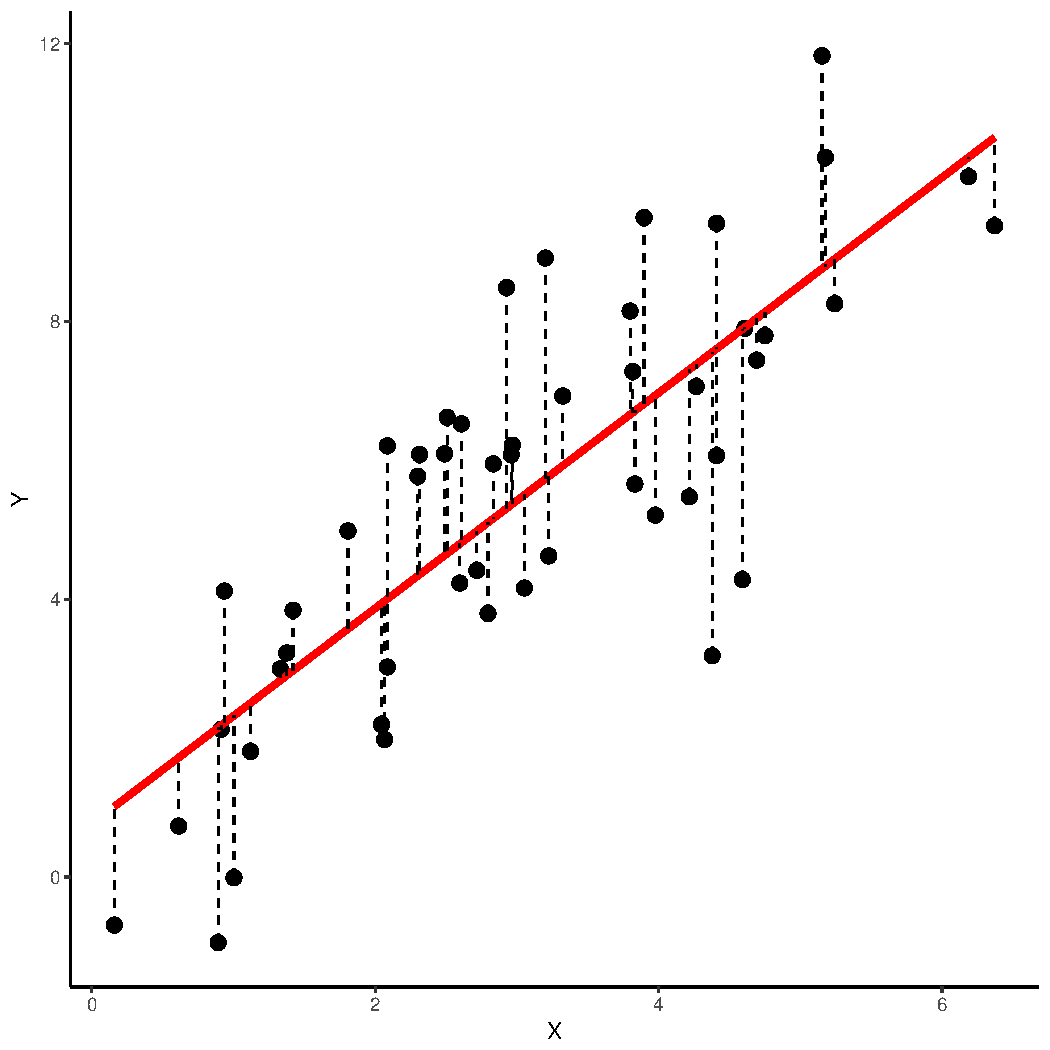
\includegraphics[height=1.75in]{bivariate-regression-image.pdf}}
\end{figure}

\smallskip

The standard bivariate regression equation relating one observed variable $X$ (the predictor) to another observed variable of interest, $Y$ (the outcome) is usually written as:
\[
\widehat{Y} = a + bX.
\]
where $\widehat{Y}$ is the predicted value of $Y$ and $a$ (intercept) and $b$ (slope) are  chosen to minimize $\sum (Y_i - \hat{Y}_i)^2$.


\end{frame}
%===========================================================


%===========================================================
\begin{frame}
  \frametitle{Geometry of Bivariate Regression}


Let's express this in vector terms, and work with mean-centered vectors so the equation becomes:

\[
\vec{\widehat{y}} = b\vec{x}
\]


Geometric interpretation of regression as projection:

\begin{center}

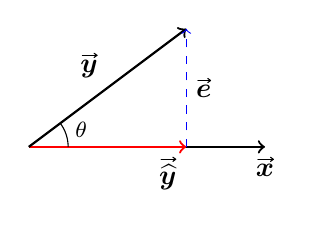
\begin{tikzpicture}[x=0.5cm, y=0.5cm]

\draw[thick,->] (0,0) -- (6,0);
\draw (6,0) node[below] {$\vec{x} $};

\draw[thick,red,->] (0,0) -- (4,0);
\draw (4,0) node[below left] {$\vec{\widehat{y}}$};

\draw[thick,->] (0,0) -- (4,3);
\draw (2,1.5) node[above left] {$\vec{y}$};

\draw[dashed,blue,->] (4,0) -- (4,3);
\draw (4,1.5) node[right] {$\vec{e}$};

\draw (0,0) +(0:0.5cm) arc (0:37:0.5cm);
\path (0,0) ++(18:0.7cm) node[font=\footnotesize] {$\theta$};

\end{tikzpicture}

\begin{gather}
\vec{\widehat{y}} = b\vec{x} \\
%
b = \frac{\vec{x} \cdot \vec{y}}{\vec{x} \cdot \vec{x}}
\end{gather}


\end{center}


\end{frame}
%===========================================================



%===========================================================
\begin{frame}[allowframebreaks]
  \frametitle{Bivariate regression: Alternate formulas for slope}

Regression equation for mean-centered vectors: $\vec{\widehat{y}} = b\vec{x}$

There are multiple, equivalent ways to write the solution for $b$:

%
\begin{align*}
b &= \frac{\vec{x} \cdot \vec{y}}{(\vec{x} \cdot \vec{x})} \\
  &= \frac{\vec{x} \cdot \vec{y}}{|\vec{x}|^2}    \\
  &= \frac{|x||y| \cos \theta}{|x|^2} \\
  &= \cos \theta \frac{|y|}{|x|} \\
  &= r_{XY} \frac{|y|}{|x|} \\
\end{align*}


\end{frame}
%===========================================================



%===========================================================
\begin{frame}
  \frametitle{Geometry of Goodness of Fit}

Geometric interpretation of regression goodness-of-fit:

\begin{center}

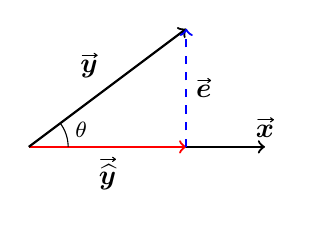
\begin{tikzpicture}[x=0.5cm, y=0.5cm]

\draw[thick,->] (0,0) -- (6,0);
\draw (6,0) node[above] {$\vec{x}$};

\draw[thick,red,->] (0,0) -- (4,0);
\draw (2,0) node[below] {$\vec{\widehat{y}}$};

\draw[thick,->] (0,0) -- (4,3);
\draw (2,1.5) node[above left] {$\vec{y}$};

\draw[thick,dashed,blue,->] (4,0) -- (4,3);
\draw (4,1.5) node[right] {$\vec{e}$};

\draw (0,0) +(0:0.5cm) arc (0:37:0.5cm);
\path (0,0) ++(18:0.7cm) node[font=\footnotesize] {$\theta$};

\end{tikzpicture}

\[
\begin{array}{c}
|\vec{\widehat{y}}|^2 + |\vec{e}|^2 = |\vec{y}|^2
\end{array}
\]

\end{center}

The better the goodness-of-fit, the smaller the angle, $\cos \theta$, and the shorter residual vector, $\vec{e}$.



\end{frame}
%===========================================================

%===========================================================
\begin{frame}
  \frametitle{Geometry of Goodness of Fit}

\begin{figure}
\begin{center}
\subcaptionbox{Good fit}{{\asyinclude[width=0.4\textwidth,keepAspect=true]{good-fit.asy}}}
\subcaptionbox{Bad fit}{{\asyinclude[width=0.4\textwidth,keepAspect=true]{bad-fit.asy}}}
\end{center}
\end{figure}

\end{frame}
%===========================================================


%===========================================================
\begin{frame}
  \frametitle{Bivariate Regression, Goodness of Fit}

How well does our prediction agree with our outcome?

\begin{itemize}
  \item Measure the angle between $\vec{\widehat{y}}$ and $\vec{y}$:
\[
R = \cos \theta_{\vec{y},\vec{\widehat{y}}} = \frac{|\vec{\widehat{y}}|}{|\vec{y}|}
\]

 \item In the single-predictor case $R = r_{XY}$, but this is not generally true when we have multiple predictors.

 \item Note that $|\vec{y}|$ can be expressed as follows:
\begin{eqnarray*}
|\vec{\widehat{y}}|^2 + |\vec{e}|^2 &=& |\vec{y}|^2 \\
SS_\mathrm{regression} + SS_\mathrm{residual} &=& SS_\mathrm{total}
\end{eqnarray*}

 \item With simple substitution we can show that:
\begin{eqnarray*}
SS_\mathrm{regression} &=& R^2 SS_\mathrm{total} \\
SS_\mathrm{residual} &=& (1-R^2)SS_\mathrm{total}
\end{eqnarray*}

\end{itemize}


\end{frame}
%===========================================================



%===========================================================
\begin{frame}
  \frametitle{Two-group ANOVA as Regression}

We can also use a geometric perspective to test whether the mean of a variable differs between two groups of subjects.

\begin{itemize}
\item Setup a `dummy variable' as the predictor $X_g$.   We assign all subjects in group 1 the value 1 and all subjects in group 2 the value -1 on the dummy variable.  We then regress the variable of interest, $Y$, on $X_g$.

\end{itemize}
%
$$
\Mtx{y} = \Mtx{X}_g\Mtx{b} + \Mtx{e}
$$
%
\begin{figure}
{\centering 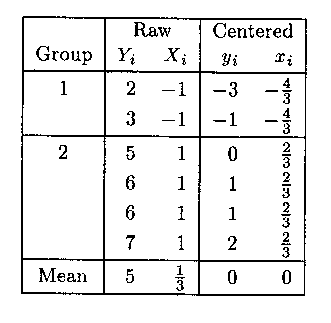
\includegraphics[height=1.5in]{anova-2group-table.pdf}}
\end{figure}


\end{frame}
%===========================================================


%===========================================================
\begin{frame}
  \frametitle{Two-group ANOVA as Regression, cont}

\begin{itemize}

\item When the means are different in the two groups, $X_g$ will be a good predictor of the variable of interest, hence $\vec{y}$ and $\vec{x_g}$ will have a small angle between them.

\item When the means in the two groups are similar, the dummy variable will not be a good predictor.  Hence the angle between $\vec{y}$ and $\vec{x_g}$ will be large.

\end{itemize}

\begin{center}

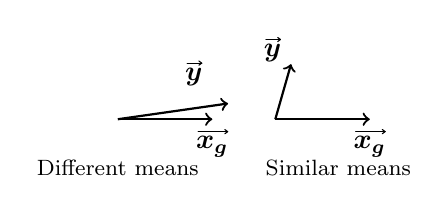
\begin{tikzpicture}[x=0.2cm, y=0.2cm]

% different means
\draw[thick,->] (-10,0) -- (-4,0);
\draw (-4,0) node[below] {$\vec{x_g}$};

\draw[thick,->] (-10,0) -- (-3,1);
\draw (-4,1.5) node[above left] {$\vec{y}$};
\draw (-10,-2) node[below,font=\footnotesize] {Different means};

% Similar means
\draw[thick,->] (0,0) -- (6,0);
\draw (6,0) node[below] {$\vec{x_g}$};

\draw[thick,->] (0,0) -- (1,3.5);
\draw (1,3) node[above left] {$\vec{y}$};
\draw (4,-2) node[below,font=\footnotesize] {Similar means};

\end{tikzpicture}

\end{center}

\end{frame}
%===========================================================



%===========================================================
\begin{frame}
  \frametitle{Introduction to Matrices}

\begin{columns}
\begin{column}{5.5cm}

\begin{itemize}
	\item One way to think about a matrix is as a collection of vectors. This is, in essence, what a multivariate data set is.

  \item A matrix which has $n$ rows and $p$ columns will be referred to as a  $n \times p$ matrix.  $n \times p$ is the shape of the matrix.
\end{itemize}

\end{column}

\begin{column}{5cm}

\[
\mathop{A}_{(n \times p)} = \left[ \begin{array}{cccc}

a_{11} & a_{12} & \cdots & a_{1p} \\
a_{21} & a_{22} & \cdots & a_{2p} \\
\vdots & \vdots & \vdots & \vdots \\
a_{n1} & a_{n2} & \cdots & a_{np} \\

\end{array}
\right]
\]

\end{column}

\end{columns}

\end{frame}

%===========================================================

%===========================================================
\begin{frame}
  \frametitle{Scalar Multiplication of a Matrix}


\begin{itemize}
	\item Let $k$ be a scalar and let $A$ be the matrix
	
\[
A = \left[ \begin{array}{cccc}

a_{11} & a_{12} & \cdots & a_{1p} \\
a_{21} & a_{22} & \cdots & a_{2p} \\
\vdots & \vdots & \vdots & \vdots \\
a_{n1} & a_{n2} & \cdots & a_{np} \\

\end{array}
\right]
\]
	

  \item then

\[
kA = \left[ \begin{array}{cccc}

ka_{11} & ka_{12} & \cdots & ka_{1p} \\
ka_{21} & ka_{22} & \cdots & ka_{2p} \\
\vdots & \vdots & \vdots & \vdots \\
ka_{n1} & ka_{n2} & \cdots & ka_{np} \\

\end{array}
\right]
\] 

\end{itemize}

\end{frame}

%===========================================================


%===========================================================
\begin{frame}
  \frametitle{Addition and Subtraction of Matrices}

\begin{itemize}
	\item Let $A$ and $B$ be matrices that have the same shape, $n \times p$:

\[
\begin{array}{cc}
A = \left[ \begin{array}{cccc}

a_{11} & a_{12} & \cdots & a_{1p} \\
a_{21} & a_{22} & \cdots & a_{2p} \\
\vdots & \vdots & \vdots & \vdots \\
a_{n1} & a_{n2} & \cdots & a_{np} \\

\end{array}
\right]

&	

B = \left[ \begin{array}{cccc}

b_{11} & b_{12} & \cdots & b_{1p} \\
b_{21} & b_{22} & \cdots & b_{2p} \\
\vdots & \vdots & \vdots & \vdots \\
b_{n1} & b_{n2} & \cdots & b_{np} \\

\end{array}
\right]
\end{array}
\]	

	
\item then
\[
A + B = \left[ \begin{array}{cccc}
a_{11} + b_{11} & a_{12} + b_{12} & \cdots & a_{1p} + b_{1p} \\
a_{21} + b_{11}& a_{22} + b_{22} & \cdots & a_{2p} + b_{2p}\\
\vdots & \vdots & \vdots & \vdots \\
a_{n1} + b_{n1}& a_{n2} + b_{n2} & \cdots & a_{np} + b_{np}\\
\end{array}
\right]
\]

\[
A - B = A + (-B)
\]

\end{itemize}

\end{frame}

%===========================================================

%===========================================================
\begin{frame}
  \frametitle{Multiplying a Matrix by a Vector}

\begin{itemize}
	\item Let $A$ be a $n \times p$ matrix, and let \Mtx{x} be a $p \times 1$ vector

\[
\begin{array}{cc}
A = \left[ \begin{array}{cccc}
a_{11} & a_{12} & \cdots & a_{1p} \\
a_{21} & a_{22} & \cdots & a_{2p} \\
\vdots & \vdots & \vdots & \vdots \\
a_{n1} & a_{n2} & \cdots & a_{np} \\

\end{array}
\right]

&	

x = \left[ \begin{array}{c}
x_1 \\ x_2 \\ \vdots \\x_p \\
\end{array}
\right]
\end{array}
\]	

	
\item then
\[
A\Mtx{x} = \left[ \begin{array}{c}
a_{11}x_1 + a_{12}x_2 + \cdots + a_{1p}x_p \\
a_{21}x_1 + a_{22}x_2 + \cdots + a_{2p}x_p \\
\vdots \\
a_{n1}x_1 + a_{n2}x_2 + \cdots + a_{np}x_p \\

\end{array}
\right]
\]

Note that $A\Mtx{x}$ is a vector with shape $n \times 1$. The $i$-the element of $A\Mtx{x}$ is equivalent to the dot product of the $i$-th row vector of $A$ with \Mtx{x}.

\end{itemize}

\end{frame}

%===========================================================

%===========================================================
\begin{frame}
  \frametitle{General Matrix Multiplication}

\begin{itemize}
	\item Let $A$ be a $n \times p$ matrix and $B$ be a $p \times q$ matrix:

\[
\begin{array}{cc}
A = \left[ \begin{array}{cccc}

a_{11} & a_{12} & \cdots & a_{1p} \\
a_{21} & a_{22} & \cdots & a_{2p} \\
\vdots & \vdots & \vdots & \vdots \\
a_{n1} & a_{n2} & \cdots & a_{np} \\

\end{array}
\right]

&	

B = \left[ \begin{array}{cccc}

b_{11} & b_{12} & \cdots & b_{1q} \\
b_{21} & b_{22} & \cdots & b_{2q} \\
\vdots & \vdots & \vdots & \vdots \\
b_{p1} & b_{n2} & \cdots & b_{nq} \\

\end{array}
\right]
\end{array}
\]	

	
\item The product $AB$ is an $n \times q$ matrix whose $(i,j)$-entry is the dot product of the $i$-th row vector of $A$ and the $j$-th column vector of $B$.

\end{itemize}

\end{frame}

%===========================================================

%===========================================================
\begin{frame}
  \frametitle{Matrix Arithmetic Rules}

\begin{enumerate}[i]
	\item $A + B = B + A$
	\item $(A + B) + C = A + (B + C)$ 
	\item $k(A + B) = kA + kB$ 
	\item $(kA)B = k(AB)$
	\item $(AB)C = A(BC)$ (associative)
	\item $A(B+C) = AB + AC$ (distributive)
	\item $(A+B)C = AC + BC$ (distributive)
\end{enumerate}

\begin{Alert}
Matrix multiplication is \emph{\textbf{not}} commutative, i.e. $AB \neq BA$ in general.
\end{Alert}

\begin{center}
\begin{footnotesize}
Be careful when you expand expressions like $(A+B)(A+B)$.
\end{footnotesize}
\end{center}

\end{frame}

%===========================================================


%===========================================================
\begin{frame}
  \frametitle{Matrix Transpose}

\begin{columns}
\begin{column}{5.5cm}

\begin{itemize}
	\item We denote the transpose of a matrix as $A^T$
	
\medskip	

  \item If $A$ is an $n \times p$ matrix, then $A^T$ is a $p \times n$ matrix where $A^T_{ji} = A_{ij}$

  \item Transpose rules:
  \begin{itemize}
  \item $(A^T)^T = A$
  \item $(A + B)^T = A^T + B^T$
  \item $(AB)^T = B^T A^T$
  \end{itemize}

\end{itemize}

\end{column}

\begin{column}{5cm}

\[
A = \left[ \begin{array}{cccc}

a_{11} & a_{12} & \cdots & a_{1p} \\
a_{21} & a_{22} & \cdots & a_{2p} \\
\vdots & \vdots & \vdots & \vdots \\
a_{n1} & a_{n2} & \cdots & a_{np}
\end{array}
\right]
\]

\[
A^T = \left[ \begin{array}{cccc}

a_{11} & a_{21} & \cdots & a_{n1} \\
a_{12} & a_{22} & \cdots & a_{n2} \\
\vdots & \vdots & \vdots & \vdots \\
a_{1p} & a_{12} & \cdots & a_{np}
\end{array}
\right]
\]

\end{column}
\end{columns}



\end{frame}

%===========================================================



%===========================================================
\begin{frame}
  \frametitle{Special Matrices}

\begin{columns}
\begin{column}{5.25cm}

\begin{itemize}

\item Zero matrix
\[
\mathbf{0} = \left[ \begin{array}{cccc}

0 & 0 & \cdots & 0 \\
0 & 0 & \cdots & 0 \\
\vdots & \vdots & \vdots & \vdots \\
0 & 0 & \cdots & 0 \\

\end{array}
\right]
\]

\item Square matrix

\footnotesize{A matrix whose shape is is $n \times n$}
\[
A = \left[ \begin{array}{cccc}

a_{11} & a_{12} & \cdots & a_{1n} \\
a_{21} & a_{22} & \cdots & a_{2n} \\
\vdots & \vdots & \vdots & \vdots \\
a_{n1} & a_{n2} & \cdots & a_{nn} \\

\end{array}
\right]
\]
\end{itemize}
\end{column}

\begin{column}{5.25cm}
\begin{itemize}
\item Ones matrix
\[
\mathbf{1} = \left[ \begin{array}{cccc}

1 & 1 & \cdots & 1 \\
1 & 1 & \cdots & 1 \\
\vdots & \vdots & \vdots & \vdots \\
1 & 1 & \cdots & 1 \\

\end{array}
\right]
\]

\item Diagonal matrix

\footnotesize{A square matrix where the off-diagonal elements are zero.}

\[
A = \left[ \begin{array}{cccc}

a_{11} & 0 & \cdots & 0 \\
0 & a_{22} & \cdots & 0 \\
\vdots & \vdots & \vdots & \vdots \\
0 & 0 & \cdots & a_{nn} \\

\end{array}
\right]
\]


\end{itemize}
\end{column}

\end{columns}

\end{frame}
%===========================================================

%===========================================================


%===========================================================
\begin{frame}
  \frametitle{Identity Matrix}

An identity matrix is a diagonal matrix, $I$, where:

\[
I = \left[ \begin{array}{cccc}

1 & 0 & \cdots & 0 \\
0 & 1 & \cdots & 0 \\
\vdots & \vdots & \vdots & \vdots \\
0 & 0 & \cdots & 1
\end{array}
\right]
\]

\begin{itemize}
 \item $IA$ = $AI$ = $A$ if $I$ and $A$ are  $n \times p$ matrices
 \item $A = I\Mtx{x}$ is a diagonal matrix where $a_{ii} = x_i$ if $I$ is an $n \times n$ matrix and \Mtx{x} is a $n \times 1$ vector.

\end{itemize}

\end{frame}


%===========================================================
\begin{frame}
  \frametitle{More Special Matrices}

\begin{description}

\item[Symmetric matrix] -- square matrix, $A$, where $A^T = A$

\item[Skew-symmetric matrix] -- square matrix, $A$, where $A^T = -A$

\item[Orthogonal matrix] -- square matrix for which $A^T A = A A^T = I$.

\end{description}

\end{frame}
%===========================================================



\end{document}
